\def\year{2019}\relax
\documentclass[letterpaper]{article} % DO NOT CHANGE THIS
\usepackage{aaai19}  % DO NOT CHANGE THIS
\usepackage{times}  % DO NOT CHANGE THIS
\usepackage{helvet} % DO NOT CHANGE THIS
\usepackage{courier}  % DO NOT CHANGE THIS
\usepackage[hyphens]{url}  % DO NOT CHANGE THIS
\usepackage{graphicx} % DO NOT CHANGE THIS
\urlstyle{rm} % DO NOT CHANGE THIS
\def\UrlFont{\rm}  % DO NOT CHANGE THIS
\usepackage{graphicx}  % DO NOT CHANGE THIS
\frenchspacing  % DO NOT CHANGE THIS
\setlength{\pdfpagewidth}{8.5in}  % DO NOT CHANGE THIS
\setlength{\pdfpageheight}{11in}  % DO NOT CHANGE THIS
\nocopyright
\graphicspath{{images/}}
\usepackage{array}
\usepackage{amsmath}
\usepackage{caption}

\pdfinfo{
/Title (Text-to-Image Generation)
/Author (Mark Wesley Harris)
}

\setcounter{secnumdepth}{2} %May be changed to 1 or 2 if section numbers are 
%desired.

% The file aaai19.sty is the style file for AAAI Press 
% proceedings, working notes, and technical reports.
%
\setlength\titlebox{2.5in} % If your paper contains an overfull \vbox too high 
%warning at the beginning of the document, use this
% command to correct it. You may not alter the value below 2.5 in
\title{Text to Image Generation}
\author{Mark Wesley Harris\\
University of Colorado Colorado Springs\\
wharris2@uccs.edu
}
\begin{document}

\maketitle

\begin{abstract}
Abstract.
\end{abstract}

\section{Introduction}
\label{sec:introduction}
Text to image generation is a largely studied problem in Computer Graphics, and 
more specifically Computer Vision.
Text-to-image generation is made possible through recent advancements in the 
intersection between Computer Graphics and Machine Learning. Researchers are 
applying the complex adaptive capabilities of neural networks to generate 
portions of the image not described directly through the text input.
Two of the most popular architectures studied are Generative Adversarial 
Networks and Transformers.

\section{Generative Adversarial Networks}
The Generative Adversarial Network (GAN)
was first proposed as a way to train a model to produce more realistic images
from noise. The vanilla GAN model works as essentially a random image generator.
The network is made up of two sub-architectures:
a generator, $G$, and a discriminator, $D$.
GANs are able to generate new images that have similar qualities to
those in the dataset on which they are trained
\cite{gans}.
A generalization of the GAN architecture is shown in Figure \ref{fig:gan}.

\begin{figure}[htbp]
	\centerline{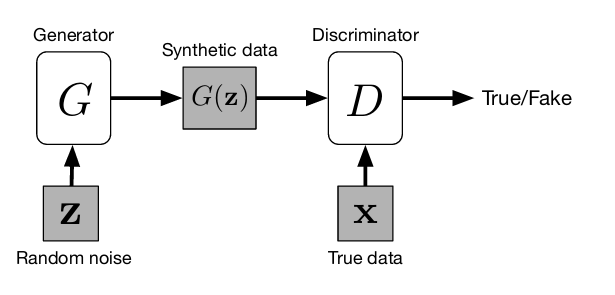
\includegraphics[width=7cm]{gan.png}}
	\caption{Basic Generative Adversarial Network architecture, with a generator $G$
		and discriminator $D$
		\cite{cgan}.}
	\label{fig:gan}
\end{figure}

The model works by training both the generator and
discriminator in tandem.
$G$ is trained to progressively generate more realistic images,
while $D$ is trained to recognize differences between real and fake inputs \cite{cgan}.
This relationship can be expressed in the format of a
``two-player min-max game'', shown in Equation \ref{eq:gan_basic}.

\begin{equation}
\label{eq:gan_basic}
\begin{split}
\text{min}_G\text{max}_DV(D,G) &=
E_{\mathbf{x}\sim p_{data}(\mathbf{x})}[\log D(\mathbf{x})] \\
&+ E_{\mathbf{z}\sim p_{z}(\mathbf{z})}[\log(1 - D(G(\mathbf{z})))]
\end{split}
\end{equation}

$p_{data}(\mathbf{x})$ represents the true data distribution,
and $p_{z}(\mathbf{z})$ represents the distribution of noise.
Optimizations and variants are based off this simple concept, of which include
the cGAN, DCGAN, and SRGAN architectures.

\subsection{Deep Convolutional Generative Adversarial Networks}
Many researchers found it difficult to train basic GANs to learn global 
structures. Many found the application of variation inference and other types 
of embedding to increase the quality of generated images \cite{varigan}.
The Deep Convolutional Generative Adversarial Network (DCGAN)
was first proposed as a way to bridge the capabilities of supervised learning 
(such as with Convolutional Neural Networks) and unsupervised learning (GANs). 
The DCGAN has a similar structure to the original GAN model, but uses 
convolutional and convolutional-transpose layers in D and G, respectively
\cite{unsupervised_learning}.

\subsubsection{Generative Adversarial Text to Image Synthesis}
\cite{gan_text_to_image}

\subsubsection{Learning Deep Representations of Fine-Grained Visual 
Descriptions}
\cite{deep_visual_descriptions}

\subsection{TBD}
\subsubsection{MSG-GAN: Multi-Scale Gradients for Generative Adversarial
Networks}
\cite{msggan}

\subsubsection{StackGAN++: Realistic Image Synthesis
with Stacked Generative Adversarial Networks}
\cite{stackgan++}

\section{Attention Mechanisms}
Attention is a technique that references past data during each iteration of 
training.
An attention function is a mapping of a query and a
set of key-value pairs to an output \cite{attention_need}.
The mathematical expression of the attention function is shown in
Equation \ref{eq:attention}.
$d_k$ is the dimension of keys and queries, and
$Q,K,V$ are matrices of queries, keys, and values, respectively.
The function uses the dot product operator, so that the output is computed as
a linear combination of weights \cite{attention_need}.

\begin{equation}
\label{eq:attention}
\begin{split}
\text{Attention}(Q,K,V) = \text{softmax}(\frac{QK^T}{\sqrt{d_k}})V
\end{split}
\end{equation}

We can model the joint probability of a sequence,
$\mathbf{x}={x_1,x_2,\dots,x_n}$,
as the product of conditional
probability distributions parameterized by a network $\theta$
\cite{generative_transformers}.
The final expression is shown in Equation \ref{eq:attention_prob}.

\begin{equation}
\label{eq:attention_prob}
p(\mathbf{x}) = \prod_{i=1}^{n}p(x_i|x_1,\dots,x_{i-1};\theta)
\end{equation}

Transformers were first proposed
as a way to use attention mechanisms more efficiently.
The Transformer relies
``\dots entirely on self-attention to compute representations of its input and 
output
without using sequence-aligned RNNs or convolution''
\cite{attention_need}.
The Encoder and Decoder for the Transformer design
are shown in Figure \ref{fig:transformer}.
An input is first encoded into the dimensional space
the Transformer works with,
and the result is then decoded back as the output of the model.
%The Transformer uses a series of attention functions to map
%between two sequences.
Transformers use a constant number of layers to model an arbitrary number of 
dependencies, which makes them useful for natural language processing and 
image 
generation
\cite{generative_transformers}.

\begin{figure}[htbp]
\centerline{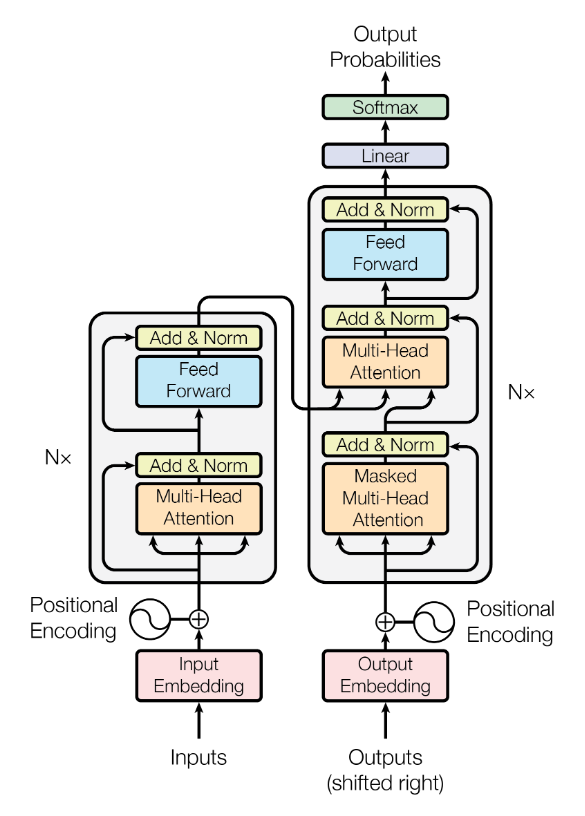
\includegraphics[width=6cm]{transformer.png}}
\caption{Transformer architecture
	\cite{attention_need}.}
\label{fig:transformer}
\end{figure}

%While the Transformer shows potential as a powerful machine learning technique,
%it is a recent concept and still has many inherent problems.
%One of the major problems with the architecture
%is that its required resources scales with $O(n^2)$
%for sequence length $n$. Researchers theorize that
%``\dots to improve computational performance for tasks involving very long 
%sequences,
%self-attention could be restricted to considering only a neighborhood of size 
%$r$''
%\cite{attention_need}.
%
%The Sparse Transformer architecture was developed as a means to shrink the
%computational resources for large sequences of data.
%Child et al. introduced sparse factorizations on the attention matrix
%in order to speed up processing.
%They approximated the dense attention
%operation by combining several cheaper attention operations.
%This new method resulted in a faster attention-based architecture
%that could be trained on longer sequences of data 
%\cite{generative_transformers}.
%
%\begin{figure}[htbp]
%\centerline{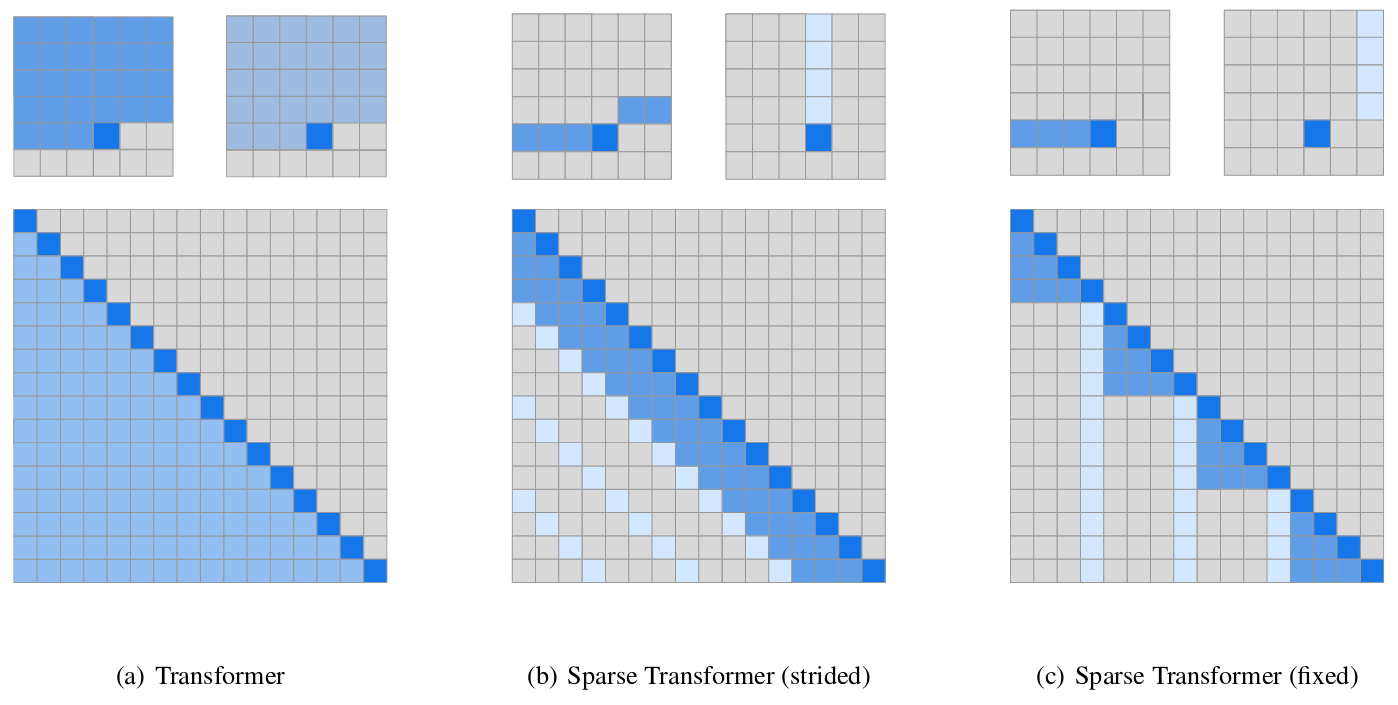
\includegraphics[width=7cm]{sparse_attention.png}}
%\caption{Optimizations of Attention
%\cite{generative_transformers}.}
%\label{fig:attention_optimization}
%\end{figure}
%
%Figure \ref{fig:attention_optimization} shows a visual representation of
%the two optimizations experimented with, strided and fixed.
%The Sparse Attention Transformer architecture reduces the resource cost to
%$O(n\sqrt[p]{n})$.
%The architecture is also simpler than other autoregressive models that perform
%similar functions, including upscaling and enhancement \cite{pixel_subscale}.

\subsection{Object-driven Text-to-Image Synthesis via Adversarial Training}
\cite{objgan}

\subsection{AttnGAN: Fine-Grained Text to Image Generation
with Attentional Generative Adversarial Networks}
\cite{attngan}

\begin{figure*}[htbp]
\centerline{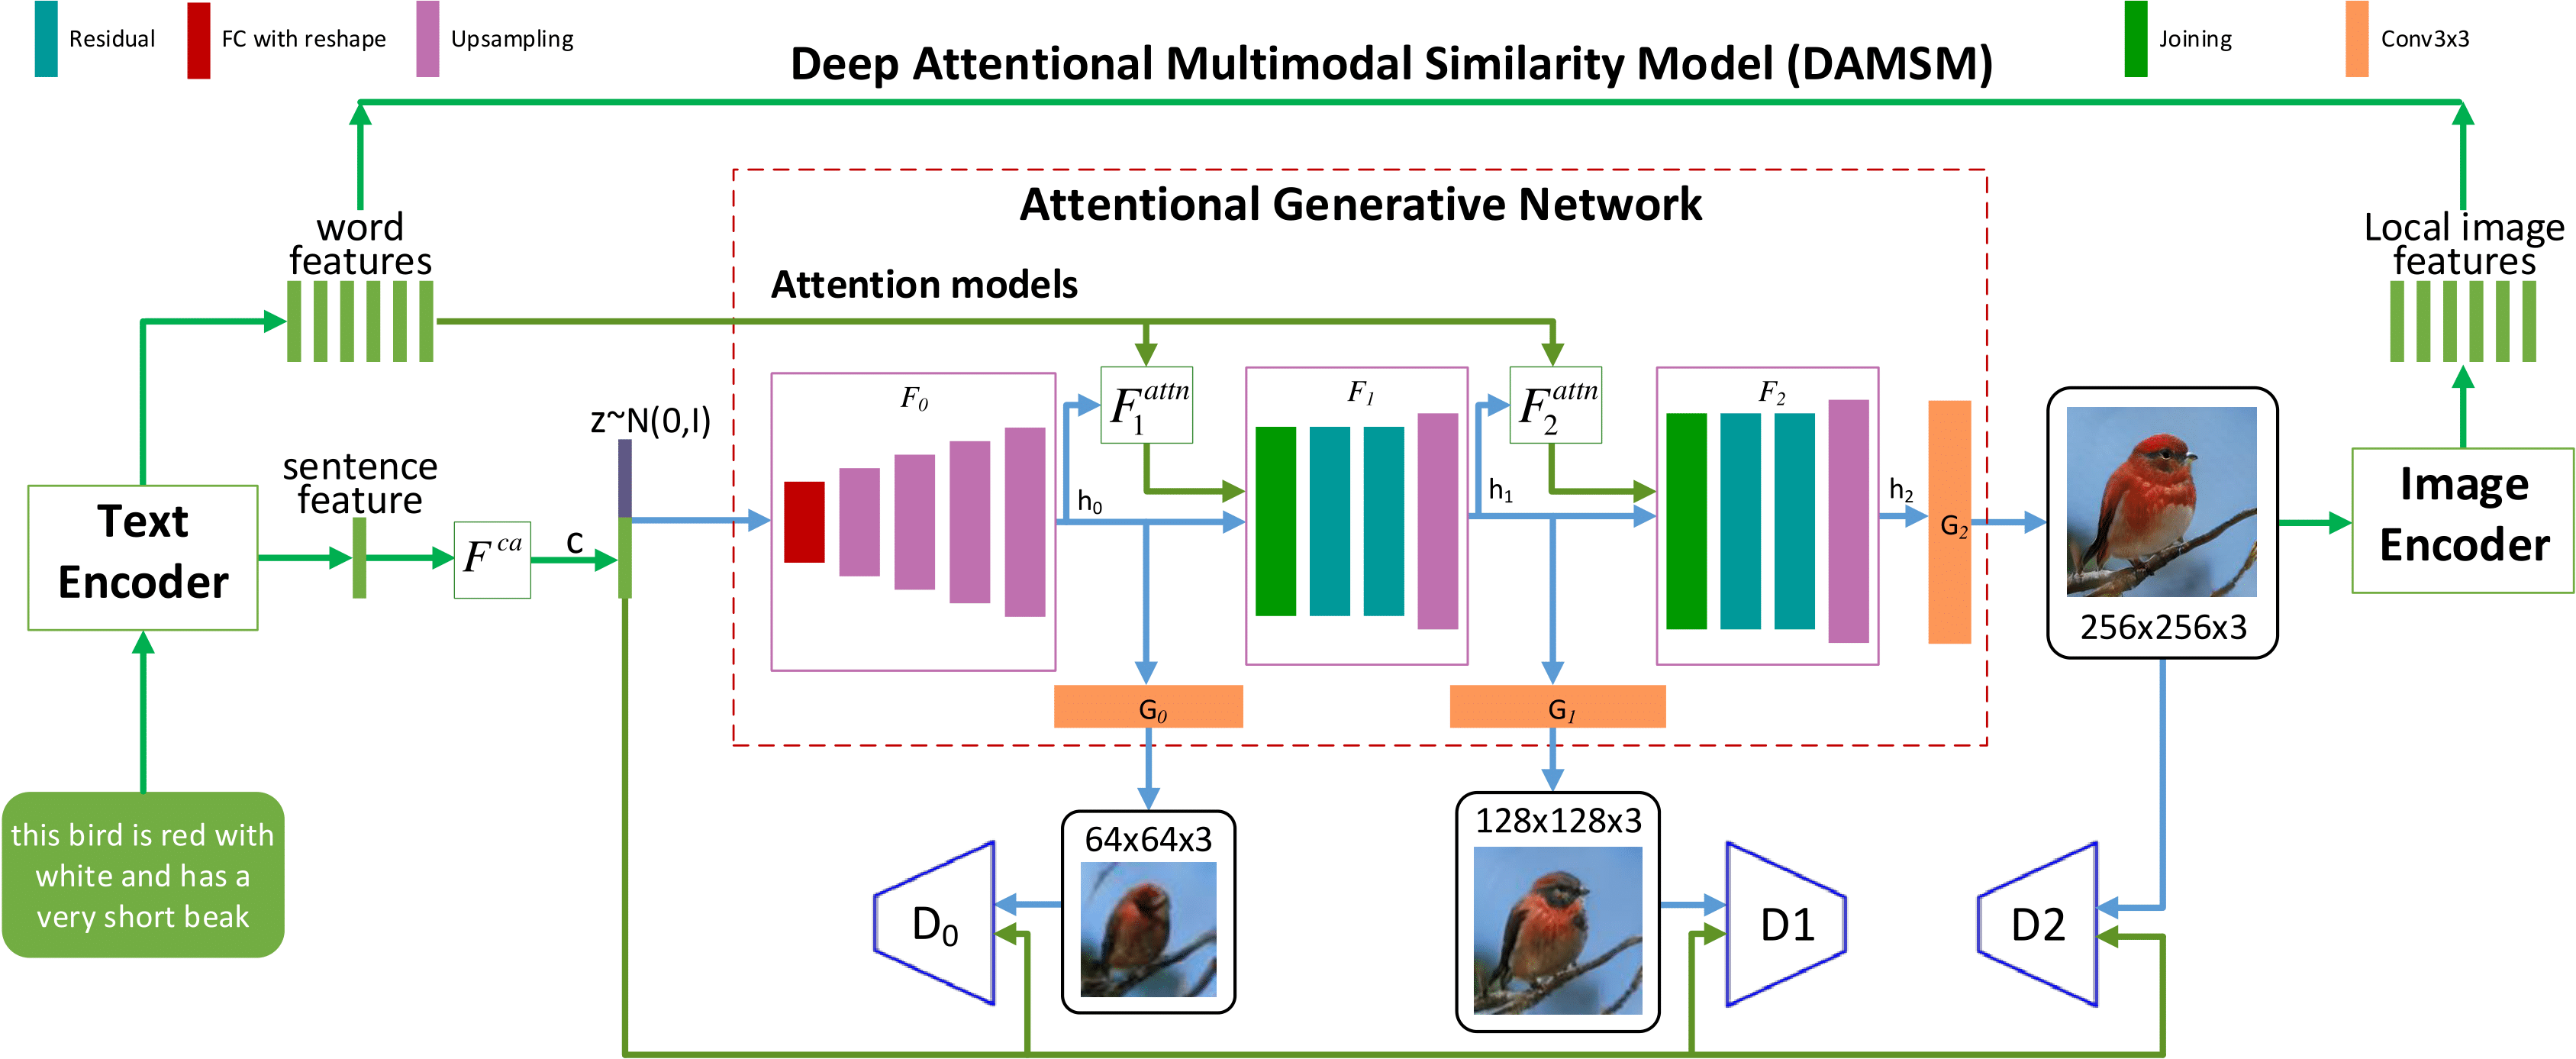
\includegraphics[width=0.95\linewidth]{attngan.png}}
\caption{.}
\label{fig:attngan}
\end{figure*}

%\subsection{Text-Guided Attention Model for Image Captioning}
%\cite{attention_caption}

\subsection{Learn, Imagine and Create: Text-to-Image Generation from Prior 
Knowledge, 2019}
\nocite{leica}
\cite{leica} combine Attention with concepts from GANs to create what they call
LEarn, Imagine and CreAte GAN (LeicaGAN). Similar to the papers discussed
previously, their architecture is comprised of a coarse image generator followed
by a fine image generator. The main difference for the LeicaGAN is their use
of textual-visual co-embedding (TVE) and multiple priors aggregation (MPA)
to further extract semantic meaning from their inputs. \cite{leica} argue that
their network more closely models how the human brain analyzes textual data,
and therefore will have better results in identifying the relationships between
an image and its textual description.

The LeicaGAN was not evaluated in the same way as the PG\textsuperscript{2} and
the VariGAN architectures; instead of converting one image to another, they
generate a novel image off of textual input alone. In this sense, the LeicaGAN
is the most relevant research to our proposed work. However, since the results
are more arbitrary, it is possible the network could fail in recognizing the
precise representations and complexities within a scene as a whole.
We propose first using the baseline AttnGAN architecture also used by 
\cite{leica}, and later applying the work from LeicaGAN and other architectures 
to try to improve our results.

%\section{Evaluation Criteria}
%A major criticism of GANs and other generative models is the
%``lack of a robust and consistent evaluation method\dots''
%\cite{gmm}.
%As opposed to other machine learning models, GANs do not optimize any kind of 
%objective function,
%and operate instead on a learned latent space
%which cannot be analyzed analytically.
%Thus, in order to evaluate the implemented models,
%we must find a way to numerically compare the generated images to their 
%respective targets.
%
%Researchers have defined many different means of comparing two images.
%Some of this research is focused on image context, such as if two images 
%contain the same
%person or setting.
%This type of analysis would not benefit our project,
%since the image needs to be exact --
%simply containing similar features is not enough.
%Thus, we turned to the measurements of
%Mean Squared Error (MSE) and Peak Signal-To-Noise Ratio (PSNR),
%as both metrics are commonly used to evaluate super resolution algorithms
%\cite{super_resolution}.

%\section{Work Completed}
%\begin{figure}[htbp]
%\centerline{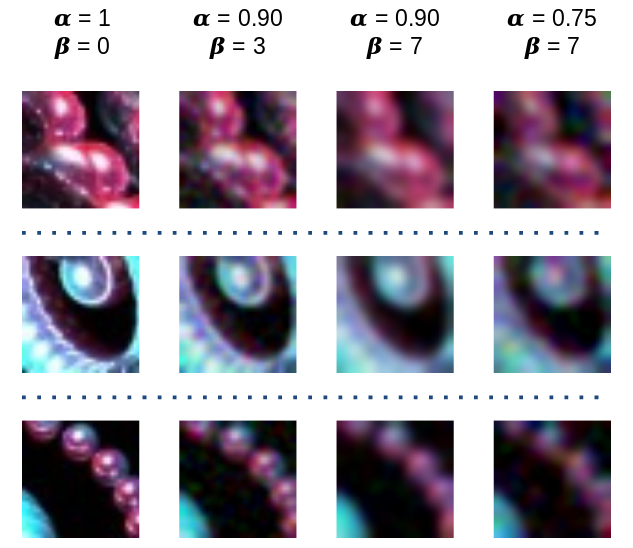
\includegraphics[width=8cm]{altered_data.png}}
%\caption{.}
%\label{fig:altered}
%\end{figure}

\bibliography{midterm}
\bibliographystyle{aaai}

\end{document}
